\documentclass[a4paper]{article}

\newcommand{\Rfunction}[1]{{\texttt{#1}}}
\newcommand{\Rpackage}[1]{{\textit{#1}}}
\usepackage{fullpage}
\usepackage{float}
\usepackage{hyperref}
\usepackage{enumerate}
\usepackage{indentfirst}

\hypersetup{
    colorlinks,%
    citecolor=black,%
    filecolor=black,%
    linkcolor=black,%
    urlcolor=blue
}
 
\title{ \Huge SeaFlow Cruise Report}
\author{
       Francois Ribalet \& Ginger Armbrust\\
       School of Oceanography\\
       University of Washington\\
       Seattle, WA 98195\\
 \href{mailto:ribalet@uw.edu}{\texttt{ribalet@uw.edu}}\\
 \href{mailto:armbrust@uw.edu}{\texttt{armbrust@uw.edu}}
 \date{}
}
\usepackage{Sweave}
\begin{document}
%\setkeys{Gin}{width=0.8\textwidth}

\maketitle

\vspace{20 mm}

\begin{center}
\large March 21 2015 \\
 -\\
\large  March 29 2015
 \end{center}

\vspace{20 mm}

\begin{figure}[h]
\centering

\includegraphics[width=0.8\textwidth]{logo.jpg}
\end{figure}		

\vspace{20 mm}

\begin{center}
Report created on \today
 \end{center}


\newpage
Copyright@2015 Francois Ribalet and Contributers. All rights reserved.
Permission is granted to copy, distribute and/or modify this document under the terms of the GNU Free Documentation License, Version 1.3 or any later version published by the Free Software Foundation; with no Invariant Sections, no Front-Cover Texts, and no Back-Cover Texts.\\

DISCLAIMER: This document has been generated in a automated fashion using \LaTeX, R \& Sweave. It is provided "as is", without any warranty whatsoever, whether express, implied, or statutory, including, but not limited to, any warranty of merchantability or fitness for a particular purpose or any warranty that the contents of the item will be error-free.

\newpage
\section{Methods}
Flow cytometry measures light scattering and fluorescence emission of individual particle at rates of up to several thousand cells per second. Light scattering is roughly proportional to the cell size, and fluorescence is unique to the emission spectra of cell pigments. These parameters allows discrimination between cells and detritus or suspended sediments and between photosynthetic and non-photosynthetic organisms.
The data presented in this report was collected using  \textbf{SeaFlow}, an underway flow cytometer designed to be deployed on oceanographic research vessels to continuously monitor phytoplankton. More information about the instrument can be found in this publication:

\begin{enumerate}[(a)]
\item{
Swalwell, J, Ribalet, F. and Armbrust, E.V.
\newblock 2011. SeaFlow: A novel underway flow-cytometer for continuous observations of phytoplankton in the ocean. \newblock \emph{Limnology \& Oceanography Methods}, 9: 466-477
}
\end{enumerate}

SeaFlow data file are written in 3-min intervals along with GPS position, the universal time constant (UTC), and any other data collected through the ship\'s network (salinity, temperature, bulk chlorophyll and par). Automated analysis and visualization of measured phytoplankton populations were performed using our software package called \texttt{popcycle}\footnote{The \texttt{Popcycle} package is licensed under the Artistic License v3.0: it is therefore free to use and redistribute, however, we, the copyright holders, wish to maintain primary artistic control over any further development.}.

For more information about the SeaFlow project, please visit our website at \url{http://seaflow.ocean.washington.edu}. 


\vspace{15 mm}
\begin{figure}[h]
\centering
\begin{minipage}{0.5\linewidth}
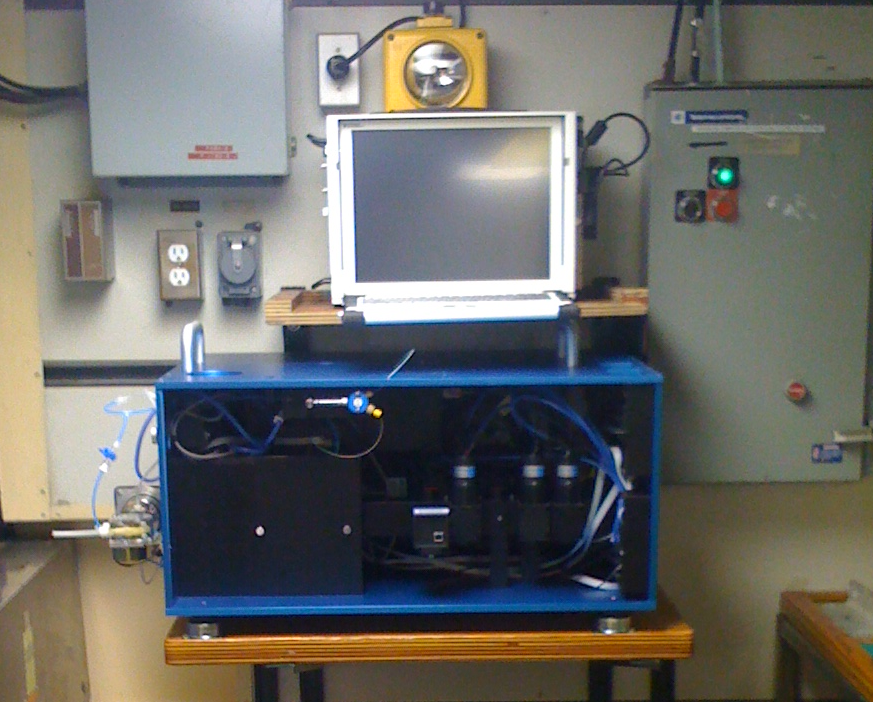
\includegraphics[width=1\textwidth]{seaflow2.png}
\caption{SeaFlow on the research vessel Thomas G. Thompson (University of Washington) in April 2010}
\end{minipage}
\end{figure}		


\newpage
\section{Results}
\subsection{Phytoplankton classification}
During the cruise, the instrument recorded a total of \texttt{3796} files from \texttt{March 21 2015} to \texttt{March 29 2015}, for a total of \texttt{8} days. The software was set up to cluster \texttt{3} phytoplankton populations. Only validated data was used to cluster a pre-defined number of phytoplankton populations. Here is a random file that shows the gates of the \texttt{3} populations.%change order of sentence or can we insert "and" into population list before crypto?


\begin{figure}[H]
\centering
%\begin{minipage}{0.8\linewidth}
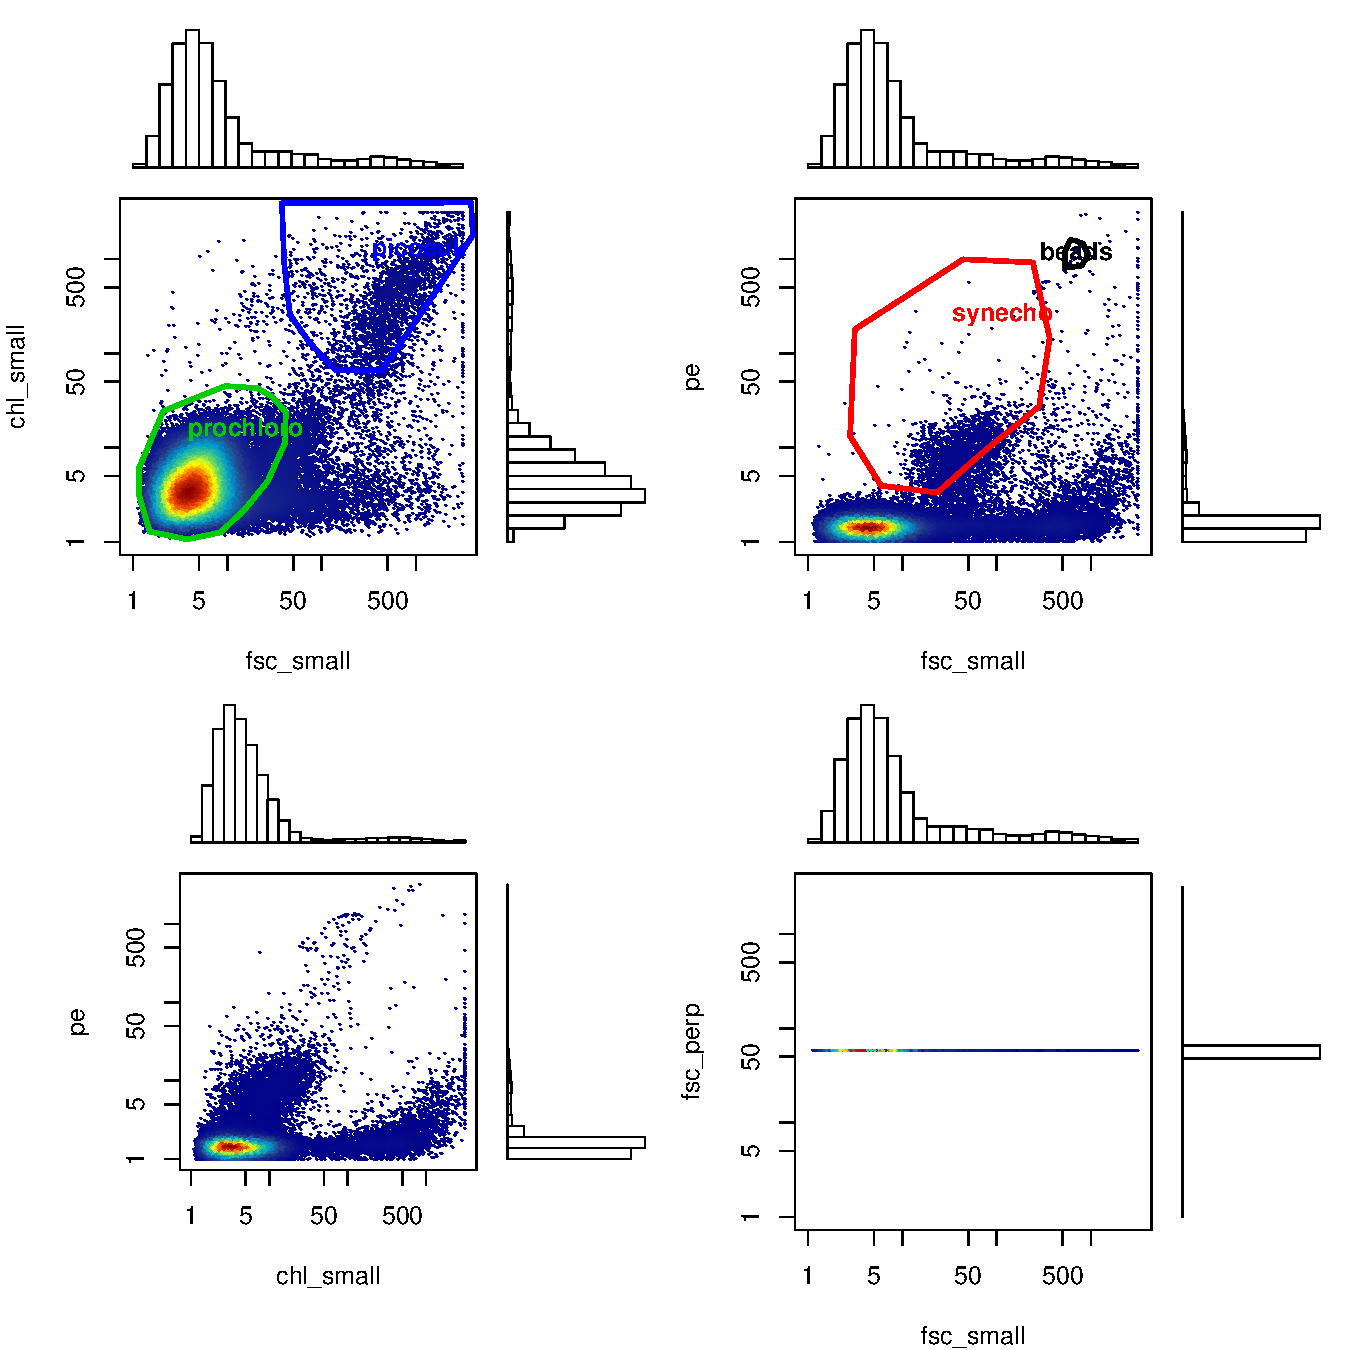
\includegraphics{CruiseReport-002}
\caption{Flow cytometric signatures of 3 phytoplankton populations: picoeuk. 'fsc\_small' represents the forward angle light scatter, which is roughly proportional to cell size; 'chl\_small' represents the red fluorescence from chlorophyll; 'pe' represents the orange fluorescence from phycoerythrin pigment and 'fsc\_perp' represents the polarized light scatter.}
%\end{minipage}
\end{figure}



\newpage
\subsection{Cell densities of phytoplankton populations}

\begin{figure}[H]
\centering
%\begin{minipage}{0.8\linewidth}
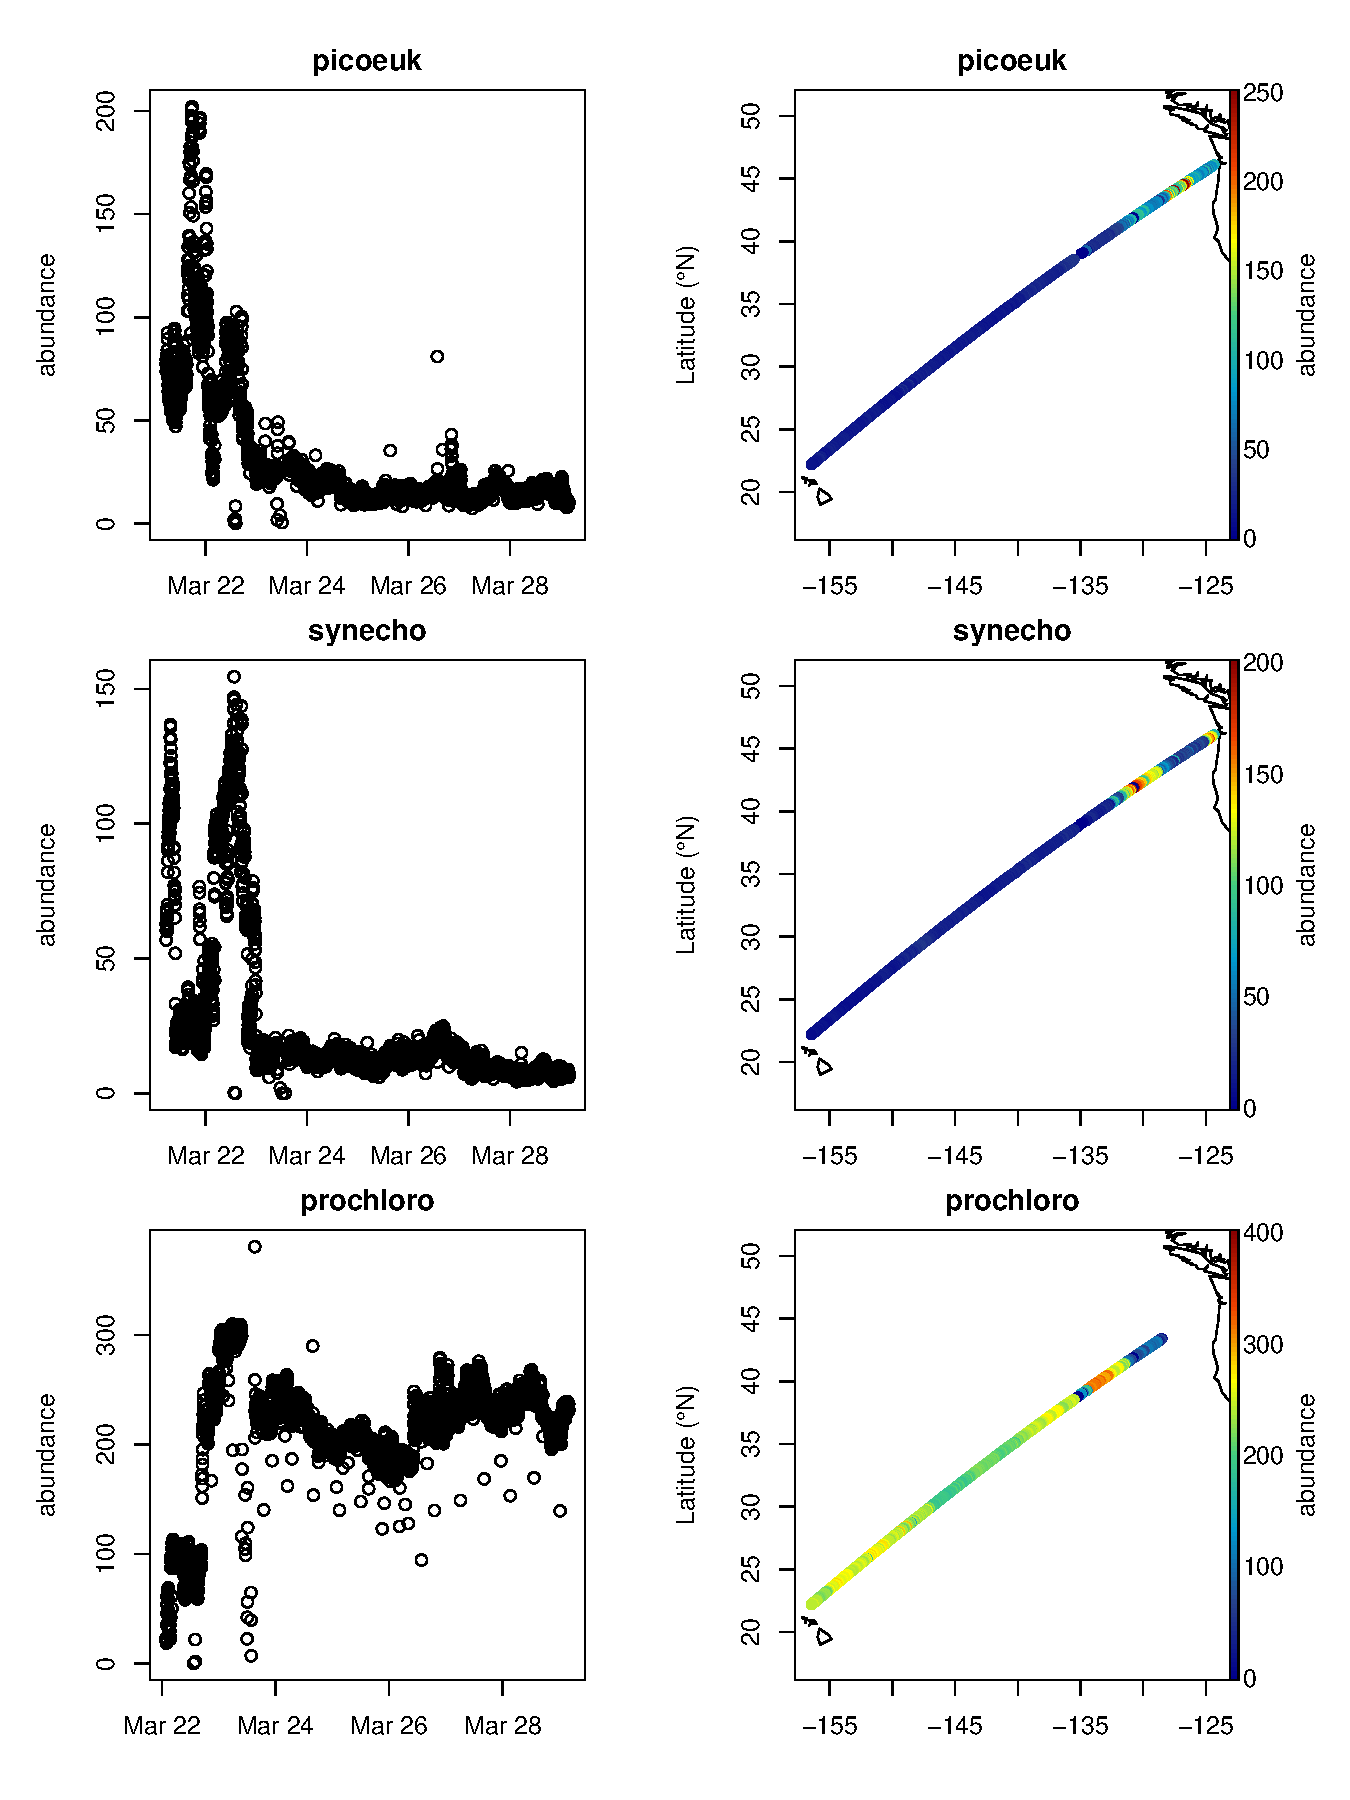
\includegraphics{CruiseReport-003}
\caption{Cell density (10$^{6}$ cells L$^{-1}$) of \texttt{picoeuk} populations plotted over time from \texttt{March 21 2015} to \texttt{March 29 2015}, and spatially.}
%\end{minipage}
\end{figure}


\newpage
\subsection{Cell Optical properties of phytoplankton populations}
\begin{figure}[H]
\centering
%\begin{minipage}{0.8\linewidth}
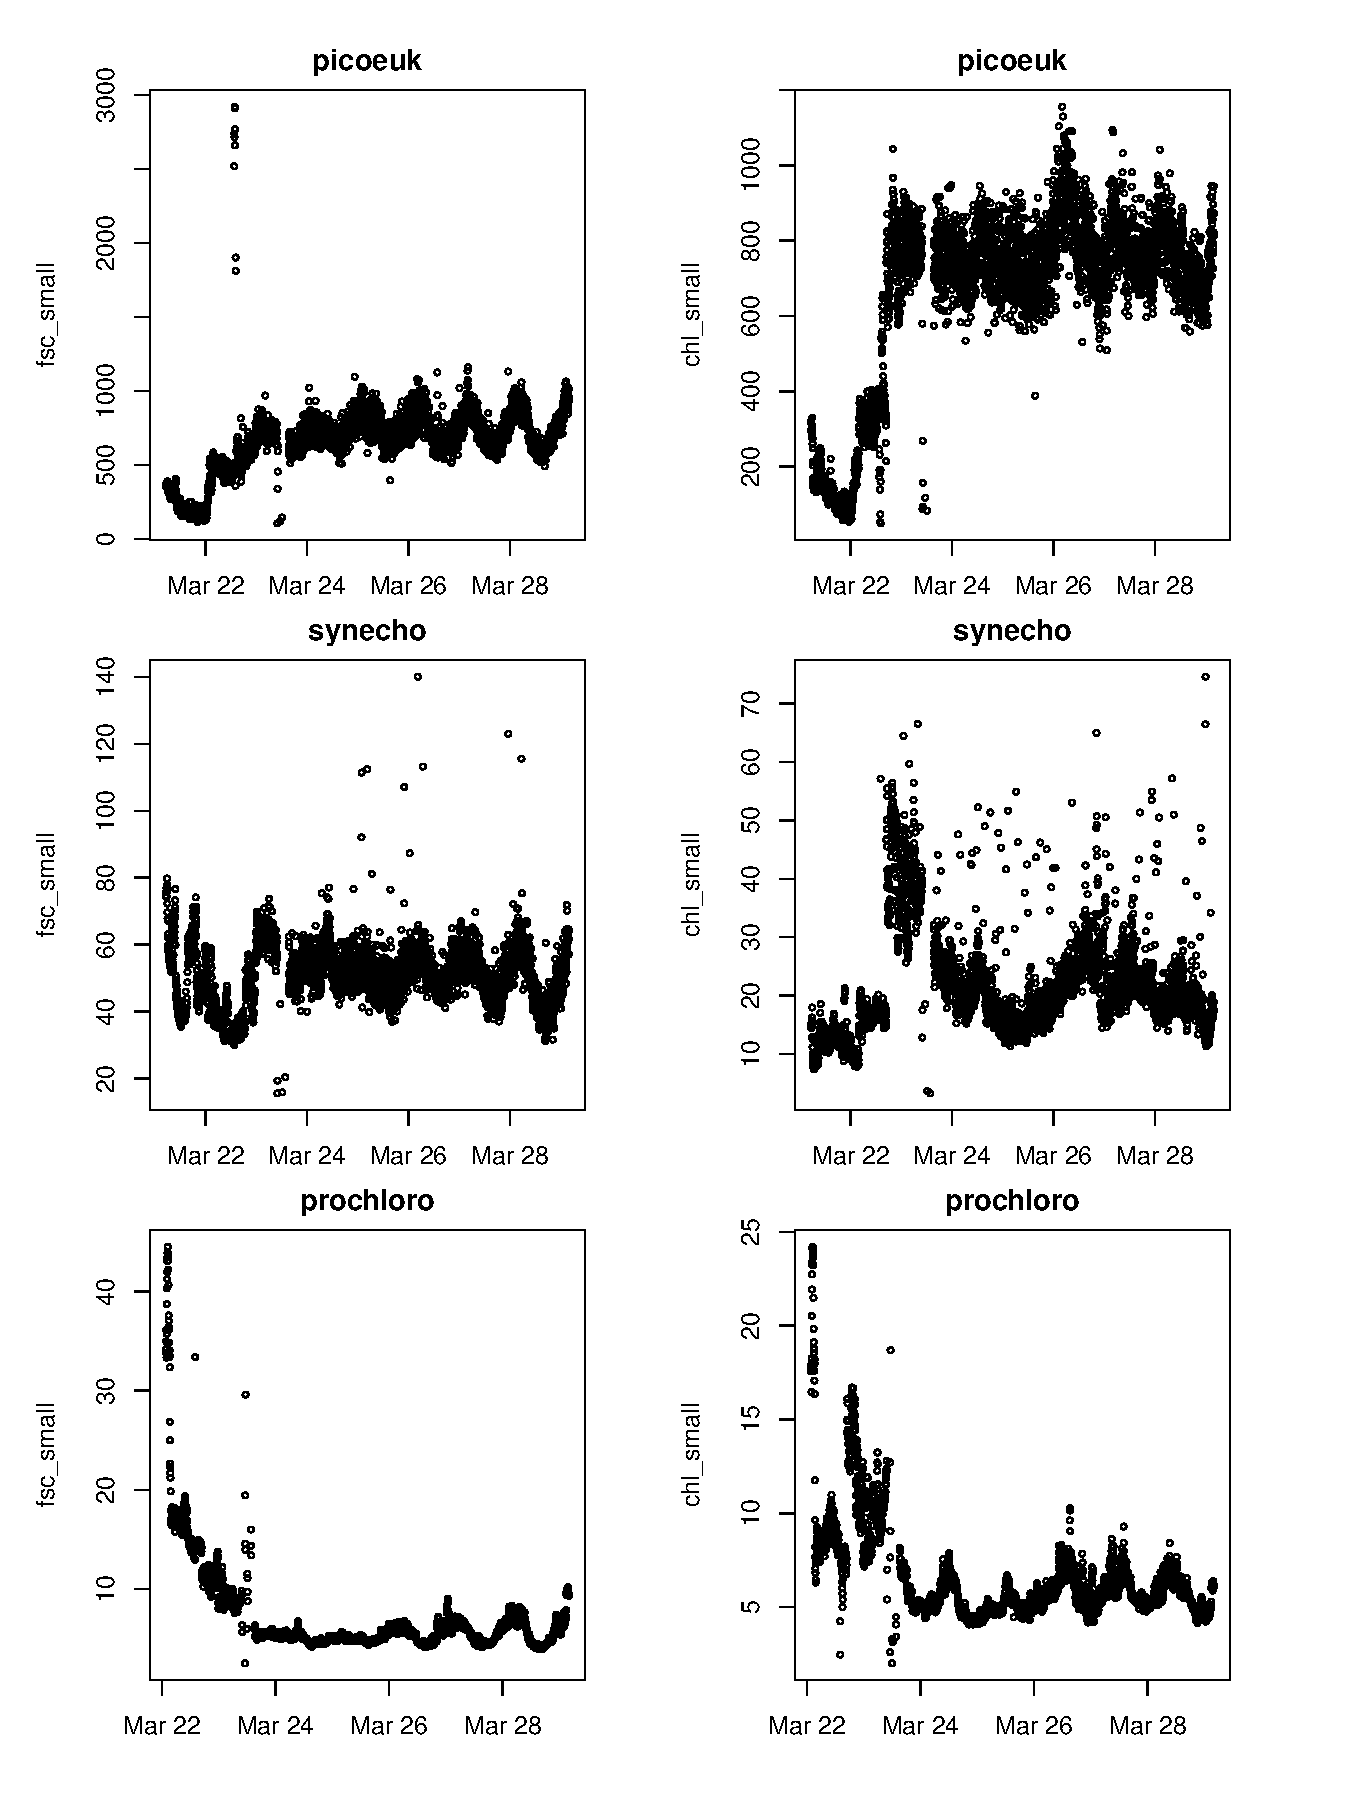
\includegraphics{CruiseReport-004}
\caption{Light scattering ('fsc\_small') and red fluorescence ('chl\_small') of the \texttt{3} identified phytoplankton populations from \texttt{March 21 2015} to \texttt{March 29 2015}.}%figure caption
%\end{minipage}
\end{figure}


\newpage
\subsection{Cytometric diversity}
The cytometry diversity indices express the organization and structure of a microbial community, its richness in physiological and genetic variations. They are based on the bio-optical properties of the community measured at the single cell level by flow cytometry. We used the \texttt{cytoDiv} R package that computes the cytometric diversity indices as described in this publication:
\begin{enumerate}[(c)]
\item{
Li, W. 1997. Cytometric diversity in marine ultraplankton.  \newblock \emph{Limnology \& Oceanography Methods}, 42: 874 - 880
}
\end{enumerate}

\begin{figure}[H]
\centering
%\begin{minipage}{0.8\linewidth}
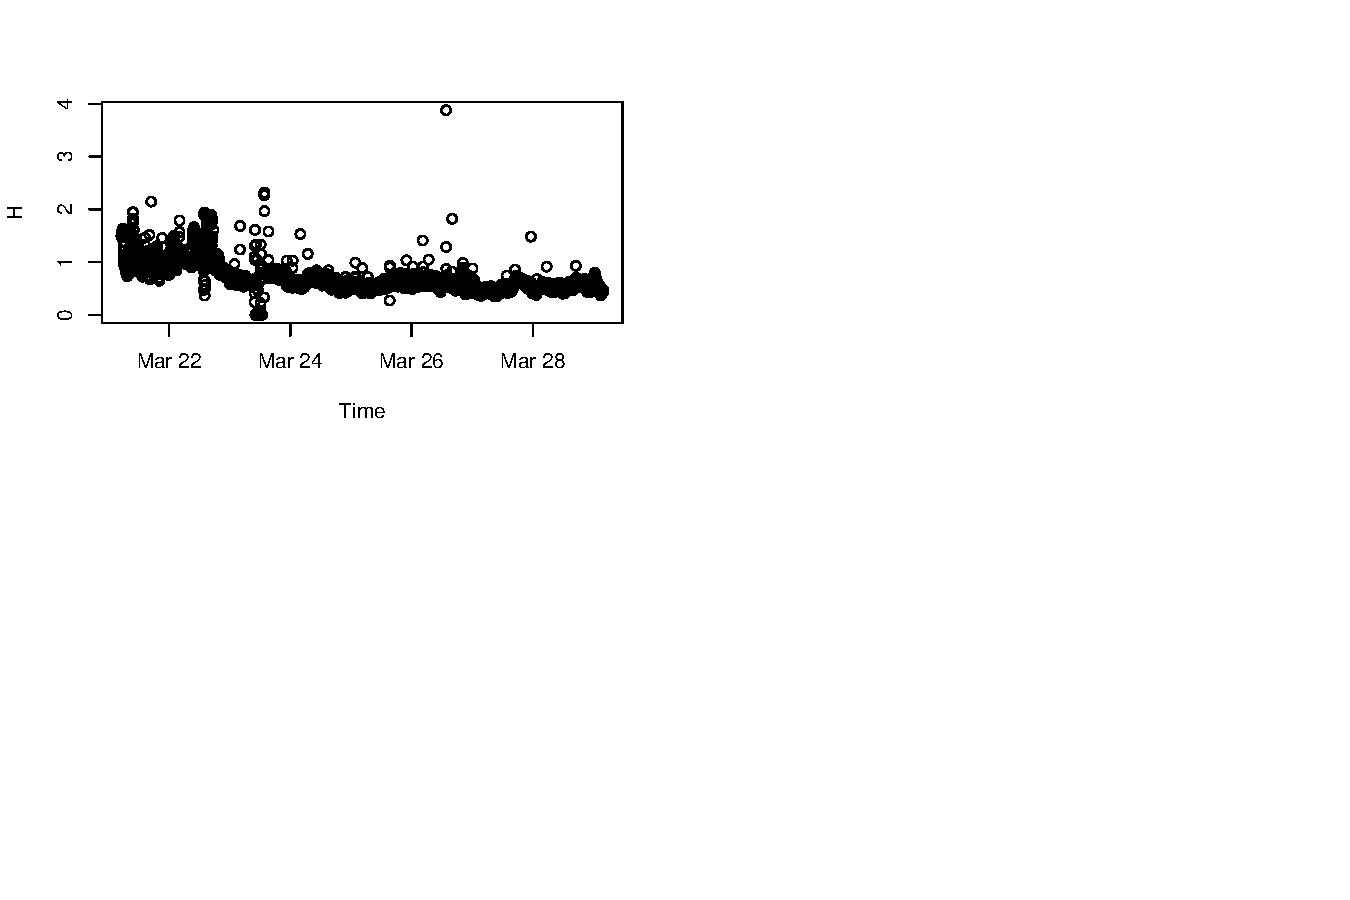
\includegraphics{CruiseReport-005}
\caption{Diversity (e$^{H}$) and Evenness (J) of the entire microbial community, plotted over time from \texttt{{March 21 2015} to \texttt{March 29 2015}}, and spatially.}%
%\end{minipage}
\end{figure}


\newpage
\subsection{Hydrographic features}
When available, SeaFlow records other underway measurements (such as temperature, salinity, bulk fluorescence and PAR) collected from the same seawater supply. WARNING these data are presented 'as-is', without calibration or any prior quality control check.

\begin{figure}[H]
\centering
%\begin{minipage}{0.8\linewidth}
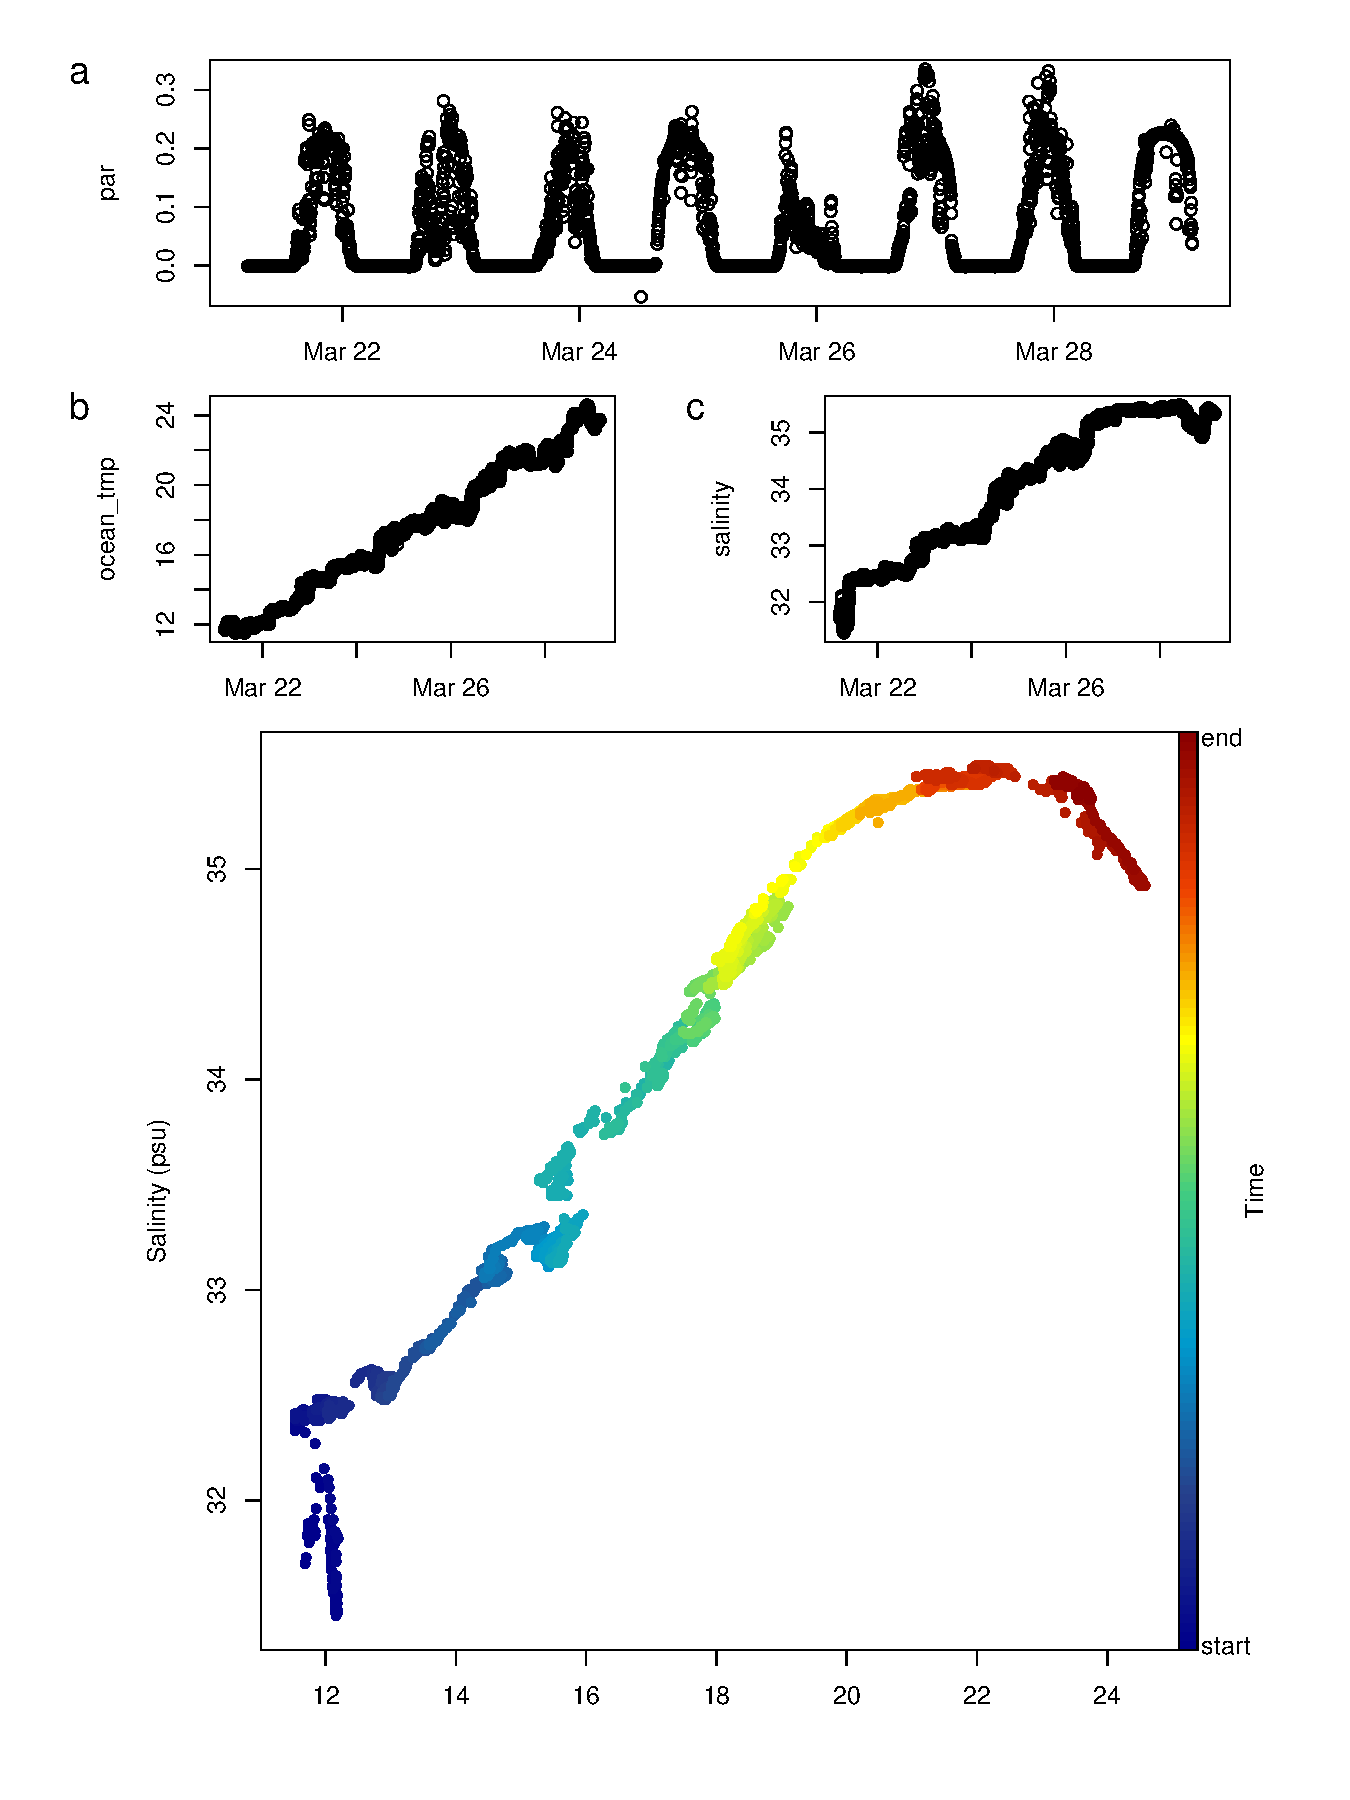
\includegraphics{CruiseReport-006}


\caption{(a) Light intensity (in arbitrary units), b) surface temperature ($\,^{\circ}\mathrm{C}$) and (c) salinity (psu) plotted over time from \texttt{March 21 2015} to \texttt{March 29 2015}, and spatially.  (d) T-S density plot with heat coloring shows progression through different water masses over time.}% units for ylab
%\end{minipage}
\end{figure}

\end{document}


